\documentclass[12pt]{beamer}
\usepackage[T2A]{fontenc}                
\usepackage[utf8]{inputenc}  
\usepackage[english, russian]{babel}
\usepackage{indentfirst}
\usepackage{graphicx}
\usetheme{Copenhagen}
\useoutertheme{infolines}
 
\begin{document}
 
\begin{frame}
    \begin{center}
        \large \textbf{Оценка стоимости опциона в биномиальной модели рынка} 
    \end{center}
    \begin{flushright}
        \bigskip \bigskip \small
        \textbf{Автор:} \\ студент 412 группы \\ Горбунов Александр Александрович \\
        \bigskip
        \textbf{Научный руководитель:} \\ к.ф.-м.н., доцент \\ Морозов Владимир Викторович
    \end{flushright}
    \begin{center}
        \bigskip \bigskip \bigskip
        \footnotesize Москва, 2019
    \end{center} 
\end{frame}
 
\begin{frame}{Цели работы}
    \begin{itemize}
        \item Оценка стоимости американского опциона в биномиальной модели рынка \\
        \item Построение аппроксимации множества немедленного исполнения американского опциона \\
    \end{itemize}
\end{frame}

\begin{frame}{Биномиальная модель рынка}
    \begin{figure}[h]
        \centering
        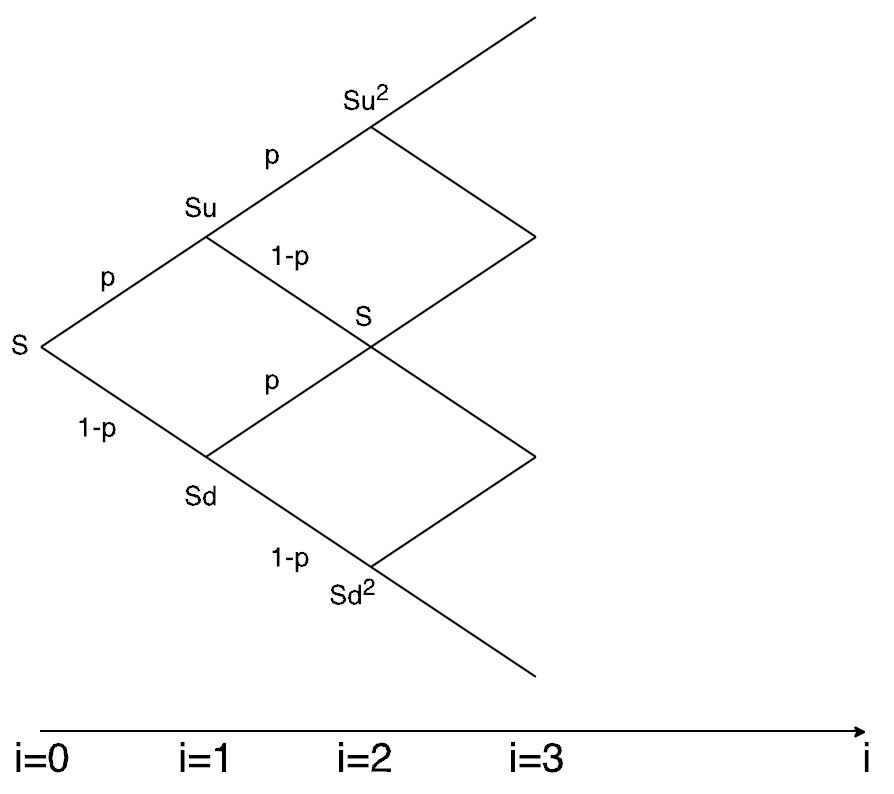
\includegraphics[scale=0.35]{scheme.jpg}
        \label{binomial}
        \caption{Изменение стоимости акции в биномиальной модели рынка с течением времени}
    \end{figure}
\end{frame}

\begin{frame}{Классический биномиальный метод}
    Оценка стоимости американского опциона осуществляется с помощью метода динамического программирования:
    \begin{equation*}
		\begin{cases}
		V_j^i = \max\,(e^{-r\Delta t} \, (pV_{j+1}^{i+1}+(1-p)V_{j-1}^{i+1}),S_j-K) \\
		V_j^n = (S_j-K)^+ \\
		\end{cases}
    \end{equation*}
    При этом стоимость самого опциона будет равна $V_0^0$.
\end{frame}

\begin{frame}{Метод Ричардсона}
    В основе метода Ричардсона лежит следующий полином:
    $$F(h)=F(0)+a_1 h^p + a_2 h^r + O(h^s), \qquad s>r>p$$
    $F(0), a_1, a_2$ - неизвестные величины.
    \begin{equation*}
        \begin{cases}
            F(h)=F(0)+a_1 h^p + a_2 h^r + O(h^s) \\
            F(kh)=F(0)+a_1 (kh)^p + a_2 (kh)^r + O(h^s) \\
            F(qh)=F(0)+a_1 (qh)^p + a_2 (qh)^r + O(h^s)
        \end{cases}
    \end{equation*}
    Цель состоит в том, чтобы отыскать $F(0)$.
\end{frame}

\begin{frame}{Метод Ричардсона}
    \footnotesize{   
        В результате, получаем, что
        $$ F(0) = F(h) + \frac{A}{C} [F(h)-F(kh)] - \frac{B}{C} [F(kh)-F(qh)],$$
        где 
        \begin{itemize}
            \item $A = q^r-q^p+k^p-k^r,$ \\
            \item $B = k^r-k^p,$ \\
            \item $C = q^r(k^p-1)-q^p(k^r-1)+k^r-k^p.$
        \end{itemize}
        Окончательно, оценка стоимости американского опциона принимает следующий вид:
        $$P = P_3 + \frac{7}{2}(P_3-P_2) - \frac{1}{2}(P_2-P_1),$$
        где $P_1=F(qh), P_2=F(kh), P_3=F(h)$, \newline $q=3,k=\frac{3}{2},p=1,r=2$.
    }
\end{frame}

\begin{frame}{Сравнительный анализ}
    \begin{table}[h]
        %\tiny
        \caption{\label{tab:Richardson}Сравнение классического биномиального метода и метода Ричардсона ($S=120, K=100, T=0.5, \sigma=0.2, r=0.03, \delta=0.07$, истинное значение опциона --- $23.710$), где K --- классический биномиальный метод, а R --- метод Ричардсона}
        \begin{table}[]
            \begin{tabular}{|l|l|l|l|l|}
                \hline
                n     & K, с.       & R, с.       & K, рез-т    & R, рез-т\\ \hline
                100   & 0.017       & 0.011       & 23.714      & 23.723       \\ \hline
                500   & 0.355       & 0.186       & 23.709      & 23.704       \\ \hline
                1000  & 1.529       & 0.740       & 23.709      & 23.705       \\ \hline
                15000 & 143.294     & 69.647      & 23.710      & 23.710       \\ \hline
            \end{tabular}
        \end{table}
    \end{table}
    Использование метода Ричардсона приводит к существенному ускорению вычисления стоимости американского опциона.
\end{frame}


\begin{frame}{Граница множества немедленного исполнения}
        \begin{figure}[h!]
            \centering
            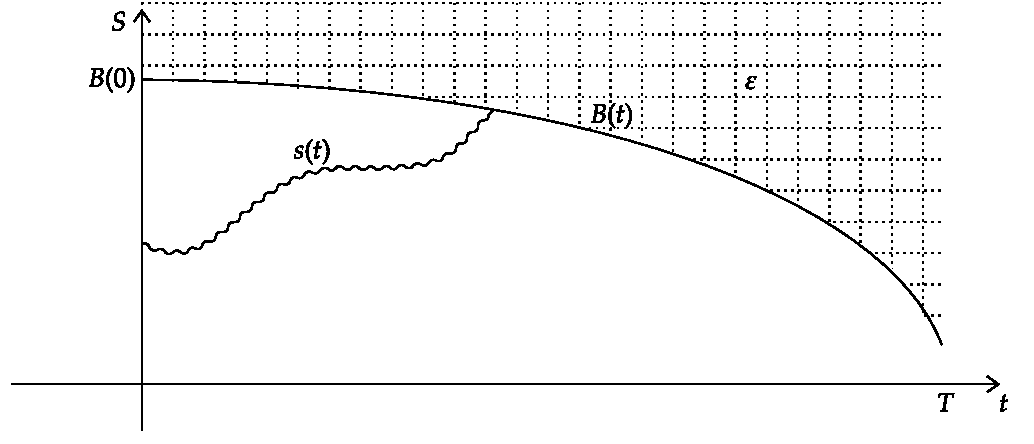
\includegraphics[scale=0.65]{Graph7.pdf}
            \caption{Граница множества немедленного исполнения $B(t)$}
            \label{boundary_of_set}
        \end{figure}
    \bigskip
\end{frame}

\begin{frame}{Метод динамического программирования}
    Граница немедленного исполнения в дискретном случае строится с помощью метода динамического программирования:
    \begin{equation*}
		\begin{cases}
		V_j^i = \max\,(e^{-r\Delta t} \, (pV_{j+1}^{i+1}+(1-p)V_{j-1}^{i+1}),S_j-K) \\
		V_j^n = (S_j-K)^+, \\
		\end{cases}
    \end{equation*}
    Значение границы в данный момент времени $i$ находится по следующему правилу:
    $$ B(i) = \sup_j \left\{ S_j \, | \, V^i_j \leq S_j - K \right\}.$$
\end{frame}

\begin{frame}{Дискретная модель}
    \begin{figure}[h]
        \centering
        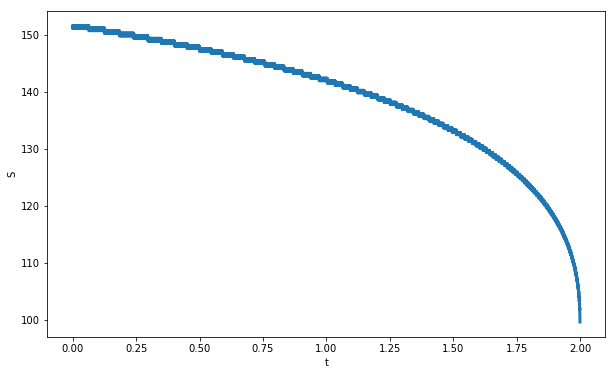
\includegraphics[scale=0.4]{Discrete.png}
        \caption{Граница области немедленного исполнения в дискретном случае при $T=2, \sigma=0.3, K=100, S=120, r=0.02, \delta=0.07$}
        \label{descrete}
    \end{figure} 
\end{frame}

\begin{frame}{Непрерывная модель}
    Требуется найти решение следующей задачи:
    $$ W'_L(S,L)\bigg|_{L=S}=0,$$
    где
    \footnotesize
    \begin{align*}
        & W'_L(S,L)\bigg|_{L=S} = \left[ 1 - \left(1-\frac{K}{S} \right)\beta_1 \right] \Phi\left(\frac{\xi\sqrt{T}}{\sigma}\right) + \\
        & + \left[ 1 - \left(1-\frac{K}{S} \right)\beta_2 \right] \Phi\left(-\frac{\xi\sqrt{T}}{\sigma}\right) + 2(a-1)e^{-\delta T} \cdot \\ 
        & \cdot \left[ \Phi\left(d_1\right) - \Phi\left(\frac{(\widetilde{\alpha}+\sigma^2)\sqrt{T}}{\sigma}\right) \right] - 2ae^{-rT}\frac{K}{S} \left[ \Phi\left(d_2\right) - \Phi\left(\frac{\widetilde{\alpha}\sqrt{T}}{\sigma}\right) \right].
    \end{align*}
\end{frame}

\begin{frame}{Непрерывная модель}
        \begin{figure}[h]
        \centering
        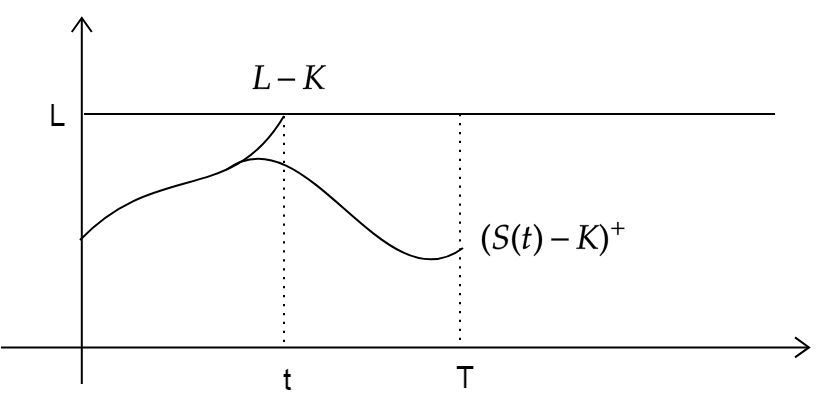
\includegraphics[scale=0.35]{Graphh1.png}
        \caption{Пояснение к расчёту среднего дисконтированного выигрыша}
        \label{demonstration}
    \end{figure}
\end{frame}

\begin{frame}{Непрерывная модель}
    \begin{figure}[h]
        \centering
        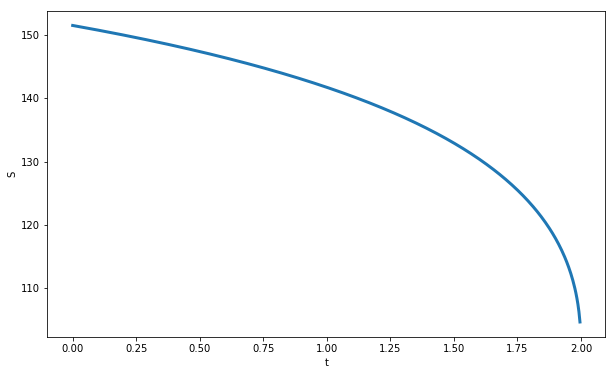
\includegraphics[scale=0.4]{Continuous.png}
        \caption{Граница области немедленного исполнения в непрерывном случае при $T=2, \sigma=0.3, K=100, S=120, r=0.02, \delta=0.07$}
        \label{continuous}
    \end{figure} 
\end{frame}

\begin{frame}{Сравнительный анализ результатов, полученных в непрерывной и дискретной моделей}
    \begin{figure}[h]
        \centering
        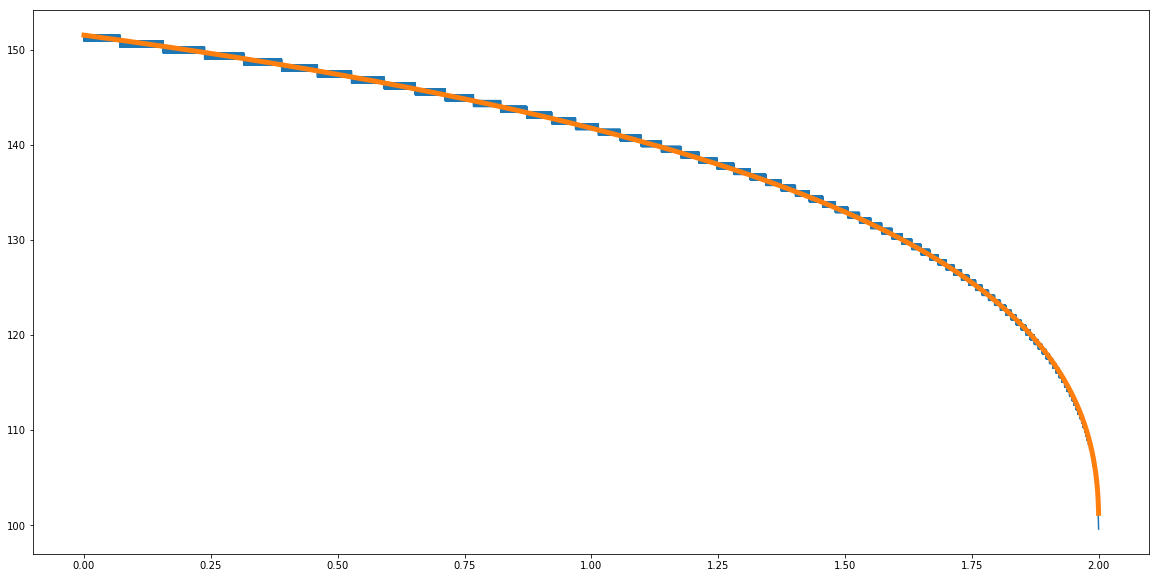
\includegraphics[scale=0.27]{Together.png}
        \label{together}
    \end{figure} 
\end{frame}

\begin{frame}{Результаты}
    \begin{itemize}
        \item Достигнуты следующие результаты:
        \begin{itemize}
            \item Построена оценка стоимости американского опциона в дискретной модели рынка;
            \item Реализован метод Ричардсона, который позволил ускорить вычисления стоимости опциона, а также показано достигаемое с его помощью ускорение;
            \item Построена аппроксимация множества немедленного исполнения американского опциона в непрерывном и дискретном случаях;
        \end{itemize}
        \item Вычисления проводились на языке \texttt{Python} в среде \texttt{Jupyter Notebook}
    \end{itemize}
\end{frame}

\end{document}

% Удалённые слайды
\begin{frame}{Постановка задачи}
    \begin{itemize}
        \item Оценить стоимость американского опциона в дискретной модели рынка \\
        \item Реализовать метод Ричардсона \\
        \begin{itemize}
            \item Показать получаемое ускорение \\
            \item Провести сравнительный анализ с классическим методом \\
        \end{itemize}
        \item Построить аппроксимацию множества немедленного исполнения американского опциона с помощью метода Броуди-Детемпла \\
        \begin{itemize}
            \item В непрерывной модели \\
            \item В дискретной модели \\
        \end{itemize}
    \end{itemize}
\end{frame}


